\chapter{Script in R}

L'esecuzione di diversi comandi ripetitivi in \texttt{R} a volte può rivelarsi 
estremamente ripetitiva, e per questo esiste la possibilità di creare quelli che 
hanno il nome di \textit{script}, ovvero corte sequenze di codice salvate in un 
file che possono essere richiamate a piacimento con un semplice comando.
La stesura di \textit{script} quindi ci aiuta la stesura di codice e ci aiuta a 
velocizzare il nostro lavoro. Per far eseguire questi \textit{snippet} sarà 
necessario usare \texttt{Rscript}, un comando da terminale apposito o 
\texttt{RStudio}, l'IDE fatto apposta per programmare in \texttt{R}.

\paragraph*{Rscript} Apriamo un terminale\footnote{Che siamo su Windows, 
GNU/Linux o MacOS non cambia} nella stessa cartella dove si trova lo script, e 
digitiamo:
\begin{lstlisting}
 Rscript -e "nomeScript.r"
\end{lstlisting}
Questo lancerà lo \textit{script} che verrà eseguito come un normale programma 
nel terminale.

\paragraph*{RStudio} Tramite \texttt{RStudio}, una volta comparsa l'interfaccia 
grafica, apriamo il nostro file scritto in \texttt{R}. Nella schermada di 
editing del file, sarà disponibile il bottone con la dicitura \textit{run}, in 
alto a destra.

\begin{figure}[h]
  \centering
  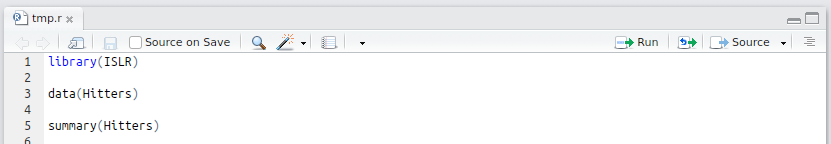
\includegraphics[scale=0.5]{RStudio}
  \caption{Un esempio di lancio di uno script da \texttt{RStudio}}
\end{figure}

\section{Scrittura}

La stesura di uno script corrisponde a come quando si danno i comandi da 
terminale, solo che questi dovranno essere trascritti in un file di testo.
